\section{M{\o}ller Polarimeter}
\label{mollerpol}

Determination of the electron beam polarization is done in Hall B using a coincidence M{\o}ller polarimeter.  The polarimeter is based 
on ${\vec e} + {\vec e}\rightarrow e + e$  elastic scattering (M{\o}ller scattering).  A detailed description of M{\o}ller scattering is presented 
in Ref.~\cite{Wagner:1990sn}.  

For a longitudinally polarized electron beam incident on a longitudinally polarized electron target, the 
center-of-momentum (CM) frame cross section is given by \cite{moller32,kresnin57}
\begin{equation}
\label{eq-csec}
 {{d\sigma}\over{d\Omega}}=
  {{d\sigma_0}\over{d\Omega}}\left(1+P_BA_{zz}P_T\right),
\end{equation}
where $d\sigma_0/d\Omega$ is the unpolarized cross section, $P_B$ and $P_T$ are the longitudinal components of the beam and target polarization, respectively, and $A_{zz}$ is the analyzing power.
The unpolarized cross section and analyzing power can be precisely calculated through QED, which gives
%
\begin{equation}
\label{eq-csecCM}
	\frac{d\sigma_0}{d\Omega}=\left(\frac{\alpha\left(3+\cos^2\theta_{CM}\right)}
						{2m_e\gamma\sin^2\theta_{cm}}\right)^2,
\end{equation}
%
and 
\begin{equation}
\label{eq-Azz}
	A_{zz}=-\frac{\left(7+\cos\theta_{CM}\right)\sin^2\theta_{CM}}{\left(3+\cos^2\theta_{CM}\right)^2},
\end{equation}
%
where $\alpha$ is the fine structure constant, $\theta_{CM}$ is the center of momentum scattering angle, $m_e$ is the electron mass, and
$\gamma=\sqrt{\left(E+m_e\right)/2m_e}$ with $E$ the lab energy of the incident electron.
From the above formulas, one sees that $A_{zz}$ has a maximum magnitude of $7/9$ at $\theta_{CM}=90^\circ$, which is the central scattering
angle for our polarimeter.

Forming the beam-helicity-dependent asymmetry gives
\begin{equation}
\label{eq-asymm}
	A=\frac{\frac{d\sigma}{d\Omega}_+-\frac{d\sigma}{d\Omega}_-}{\frac{d\sigma}{d\Omega}_++\frac{d\sigma}{d\Omega}_-}
	=A_{zz}\left(\theta_{CM}\right)P_B^zP_T^z,
\end{equation}
where the $\pm$ refers to cases where the beam helicity and the target polarization are aligned or anti-aligned.
The asymmetry can be measured from the yields according to
%
\begin{equation}
\label{eq-asymm-meas}
	A=\frac{N_+-N_-}{N_++N_-}=\langle A_{zz}\rangle P_B^zP_T^z,
\end{equation}
%
where $\langle A_{zz}\rangle$ is the effective analyzing power corrected for the finite-angle acceptance of the polarimeter and atomic-electron
motion (also known as the Levchuk effect \cite{levchuk94}).


The CLAS12 M{\o}ller polarimeter detects the scattered electrons in coincidence near $\theta_{CM}=90^\circ$, the peak of $A_{zz}$.  
The coincidence method has the advantage, as compared to 
single-arm M{\o}ller polarimetry, of producing a clean data set without having to do 
energy-dependent background subtractions (see, for example Ref.~\cite{arrington92}). Accidental background rates are typically less than
$10\%$ of the real coincident rate for our polarimeter. The accidental rate is measured and included as a correction.

\subsection{Polarimeter Design}
\label{sec-PolDesign}

The layout for the polarimeter is shown in Fig.~\ref{fig-PolLayout}. The essential elements of the polarimeter include a polarized target 
system, a pair of quadrupole magnets both operated in a dispersive mode to separate the scattered electrons from the unscattered  
beam electrons, a pair of detectors, and lead shielding between the second quadrupole and the detectors to reduce 
background.  The detectors consist of scintillating fibers packed with lead powder to form a 15.6-cm wide, 9.0-cm high, and 25-cm deep 
block with a light guide and are read out with a PMT. The detectors are surrounded by 
lead bricks with a scattered-particle aperture of 7.62 cm in the horizontal direction and 5.0 cm in the vertical direction.
The locations of the quadrupoles and detectors along with the quadrupole fields were determined by simulations of the layout. The 
locations and fields were adjusted in the simulation so that $\theta_{CM}=90^\circ\pm (4^\circ-4.5^\circ)$.

\begin{figure*}[hbtp]
 \begin{center}
  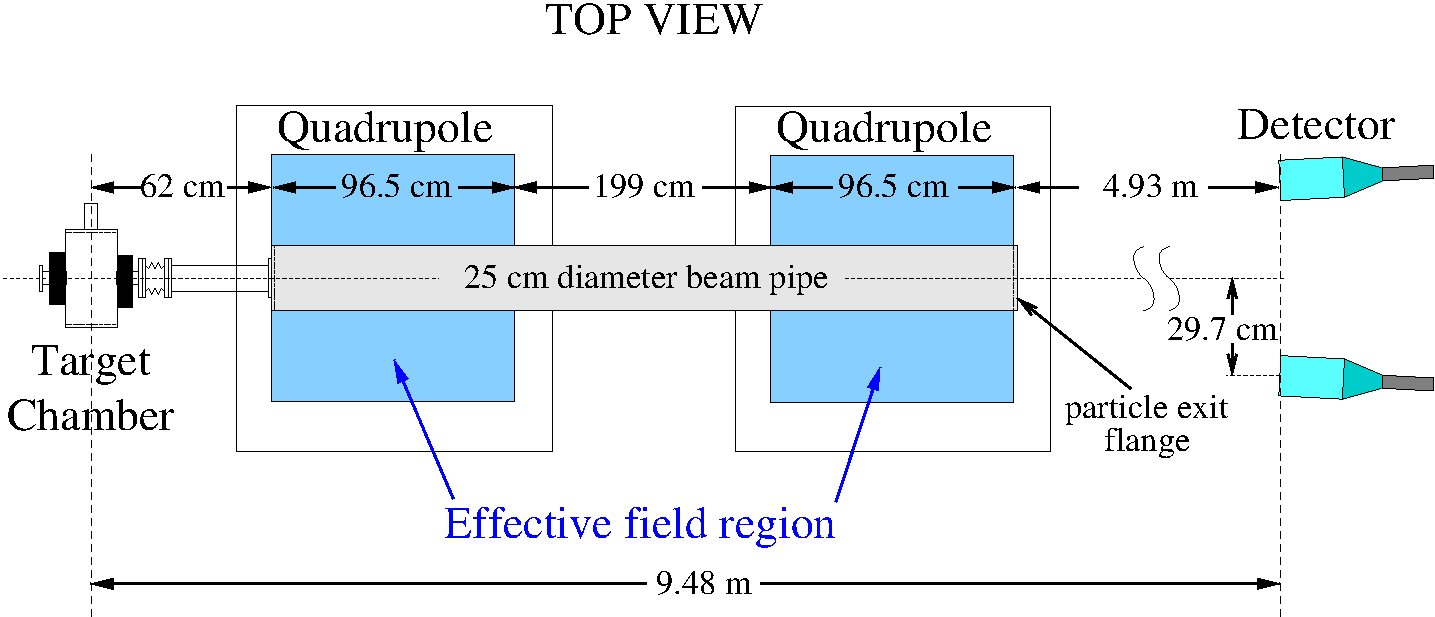
\includegraphics[width=\textwidth]{MPLayout.pdf}
 \end{center}
 \caption[]{Layout of the CLAS12 M{\o}ller polarimeter. Detector shielding is not shown.}
 \label{fig-PolLayout}
\end{figure*}


\subsubsection{Polarimeter Target}
\label{sec-PolTgt}

The target system has a pair of 25-$\mu$m-thick permendur foils on a remotely controlled insertion table housed in a vacuum 
chamber, as shown in Fig.~\ref{fig-MPtgt}. Permendur is an iron-cobalt alloy (49\% Fe, 49\% Co, 2\% Va) that has a maximum saturated polarization
of approximately 8\% along the plane of the foil when subjected to a magnetic field of greater than about 40 G. To create a longitudinally 
polarized target, the plane of a foil is 
oriented at $\pm 20^\circ$ relative to the beamline and subjected to a longitudinal magnetic holding field produced by a pair of Helmholtz 
coils on either side of the target chamber. Since only the longitudinal component of the polarization contributes to the
measured asymmetry, the target polarization used in Eq.~\ref{eq-asymm-meas} is $P_T^z=P_T\cos 20^\circ$. The $ 20^\circ$ tilt angle of the 
target maximizes the longitudinal component of the polarization while keeping mounting hardware out of the beam.

\begin{figure}[hbtp]
 \begin{center}
  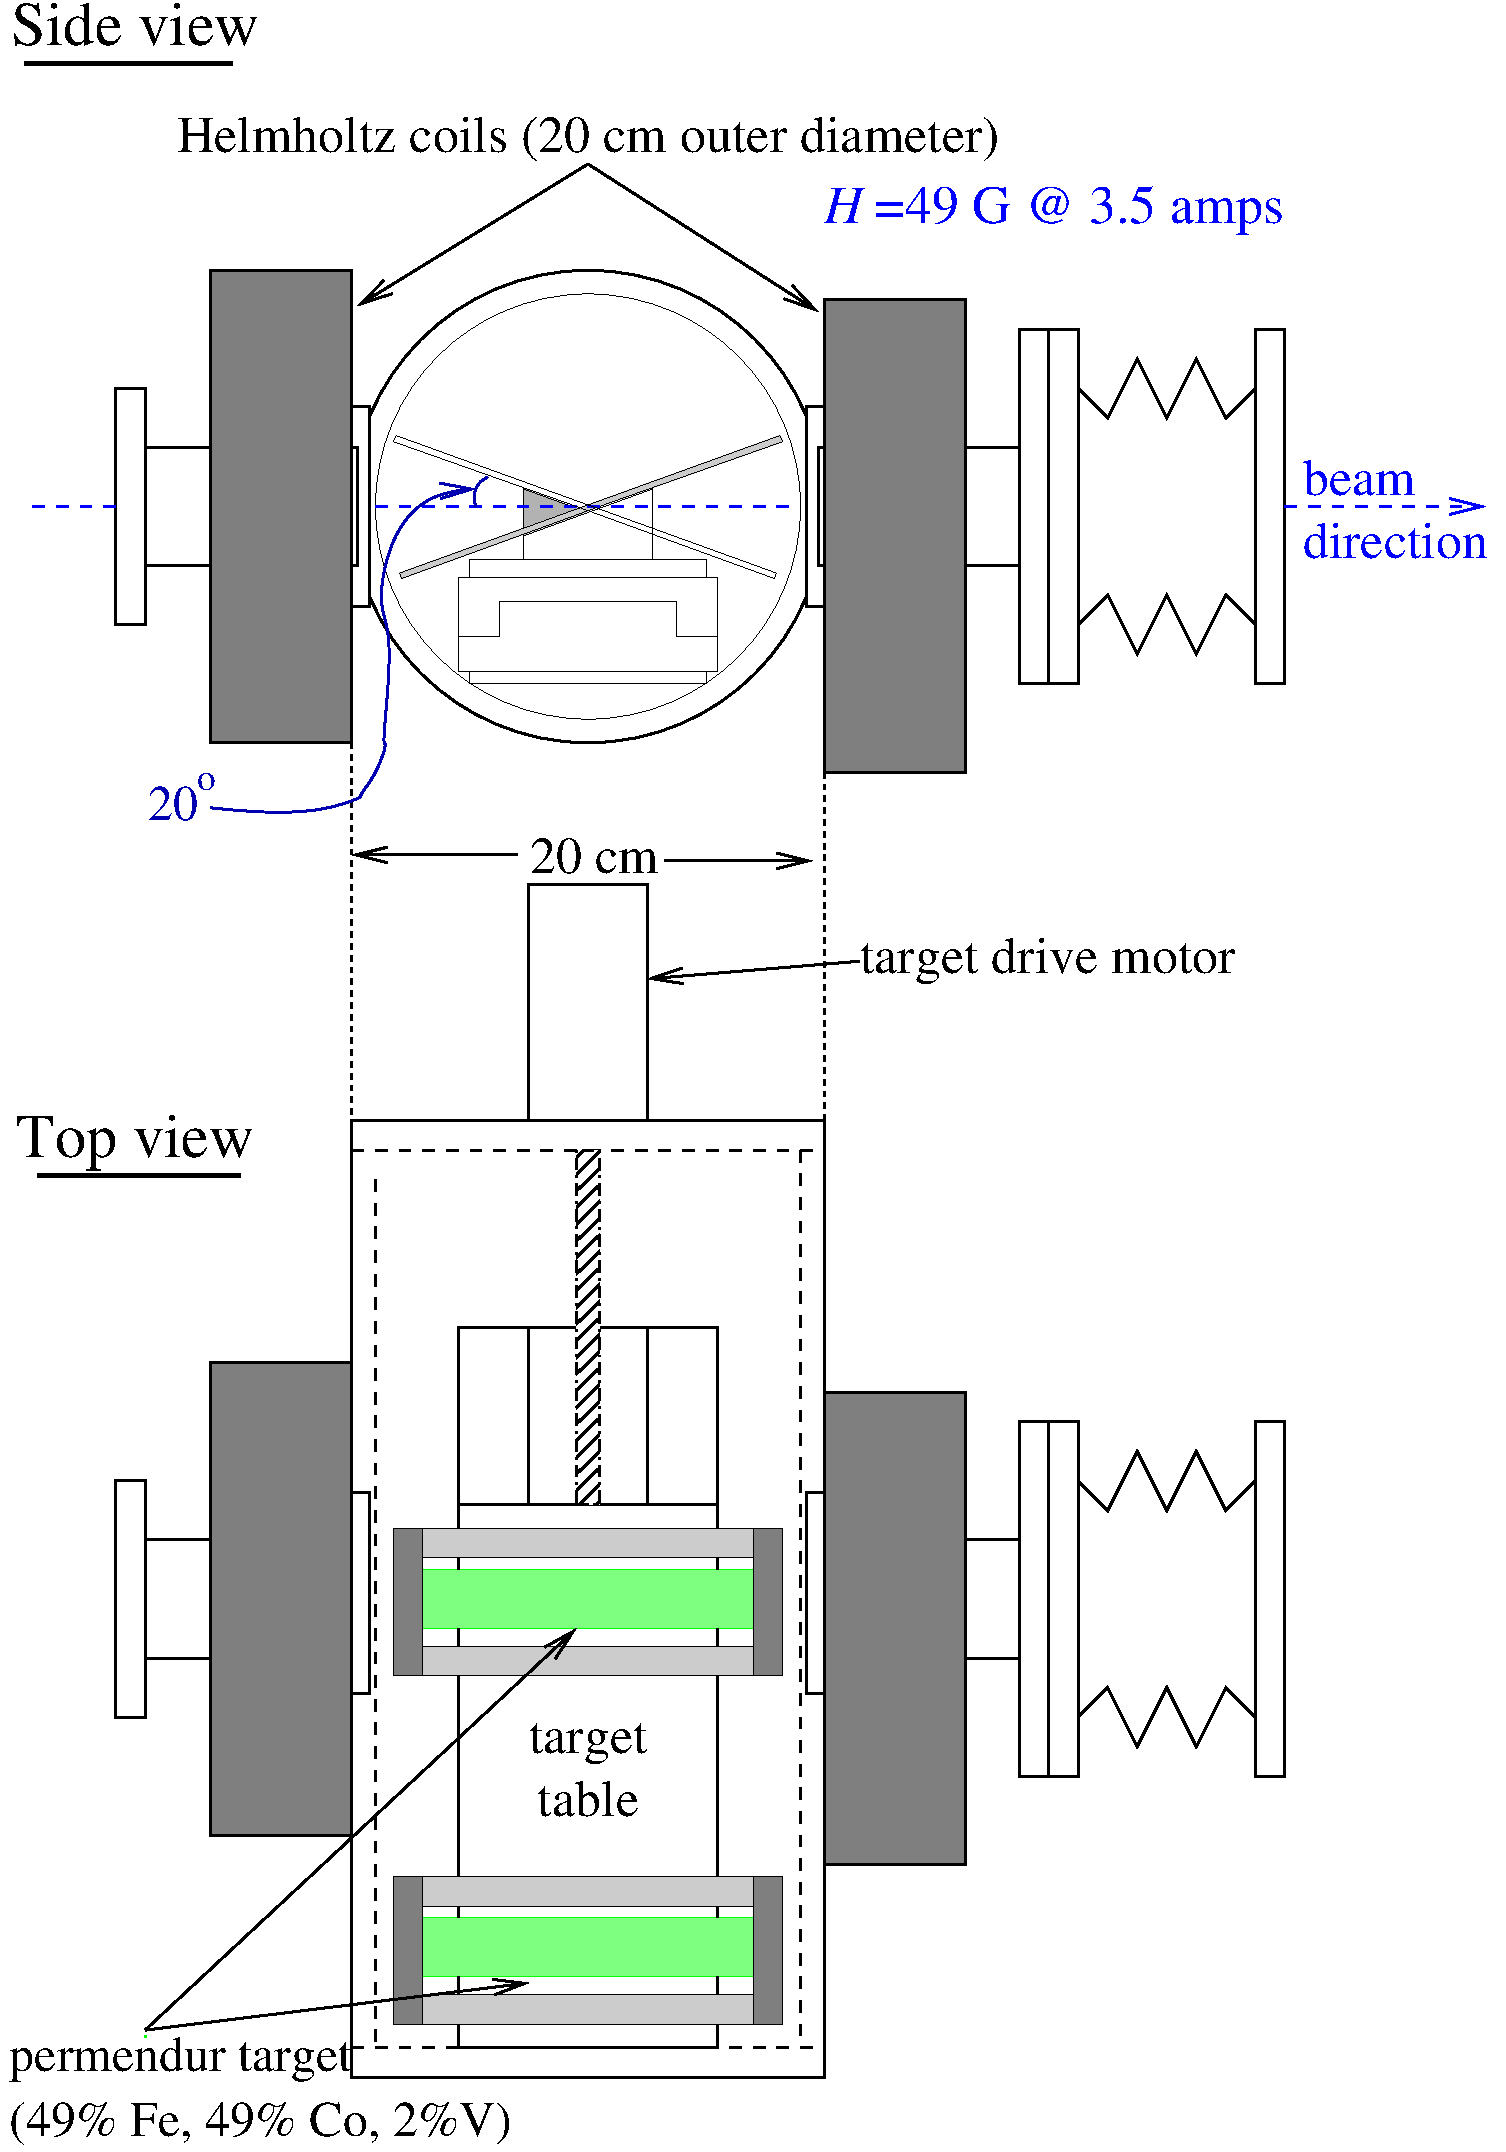
\includegraphics[width=0.5\textwidth]{MPtgt.pdf}
 \end{center}
	 \caption[]{Layout of the CLAS12 M{\o}ller polarimeter target chamber. Shown with the beam-left target inserted.}
 \label{fig-MPtgt}
\end{figure}

The polarization of the permendur target is related to the magnetization, $M$, of the foil by \cite{Band:1997ee} 
%
\begin{equation}
\label{eq-M2Pt2}
	P_T=M\left(4.546\times 10^{-5}\pm 2.9\times 10^{-7}\right),
\end{equation}
%
where $M$ is measured in units of G. The foil magnetization is measured in a separate setup consisting of a solenoid coil used to produce 
the magnetizing field, $H$, into which the target foil is placed and a pickup coil that is located at the center of the foil. A fixed current is 
applied to the solenoid to polarize the target. The direction of the current is then flipped over a time period of ~0.15 s leading to an 
induced voltage across the pickup coil. A typical pickup-coil signal is shown in Fig.~\ref{fig-TPolMeas}, which was measured with a 
digital storage oscilloscope. The flat part of this signal (highlighted by the black constant fit) corresponds to the changing applied field while 
the narrow peak in the middle of the signal results from the change in the target foil magnetization. Applying Faraday's law to the flat part of 
the signal (using the fit to interpolate under the peak) yields
%
\begin{equation}
\label{eq-H}
	\int_H  Vdt=2HN_T \langle A_{\rm coil}\rangle\rightarrow H=\frac{\int_H Vdt}{2N_T\langle A_{\rm coil}\rangle} ,
\end{equation}
%
where $\int_H Vdt$ is the area under the pickup coil signal excluding the peak, $N_T$ is the number of turns in the pickup coil, and 
$\langle A_{\rm coil}\rangle$ is the average cross-sectional area of the pickup coil.


The target polarization is related to the difference between the total area, $\int_{\rm total} Vdt$, of Fig.~\ref{fig-TPolMeas} and the area 
leading to $H$ and is given by \cite{Band:1997ee} 
%
\begin{equation}
\label{eq-PT}
	P_T=\left(1.474\pm0.010\right)l\frac{\left({\int_{\rm total} Vdt-\int_HVdt}\right)}{mN_T},
\end{equation}
%
where  $l$ is length of the target in cm, and $m$ is the mass of the target in grams with both areas measured mVs. 
Figure~\ref{fig-PSat} shows a typical saturation curve for the target, i.e.~how 
the target polarization depends on the applied field. Measurements were done with two different pickup coils with the difference between 
the two results indicating the systematic uncertainty associated with knowledge of the pickup coil geometry. For this foil, the polarization
saturated at a value of $P_T=6.17\pm 0.047$\%, where the uncertainty is a combination of the statistical uncertainties from the linear fits of 
the saturation region of the curves and the variation between the two measurements. Additional uncertainties associated with the leading 
factor in Eq.~\ref{eq-PT}, the other measured quantities in Eq.~\ref{eq-PT}, estimated variations in the target material thickness, and the 
uncertainty in the target angle relative to the beam leads to a total relative uncertainty $\delta P_T^z/P_T^z=0.014$.



\begin{figure}[ht]
 \begin{center}
  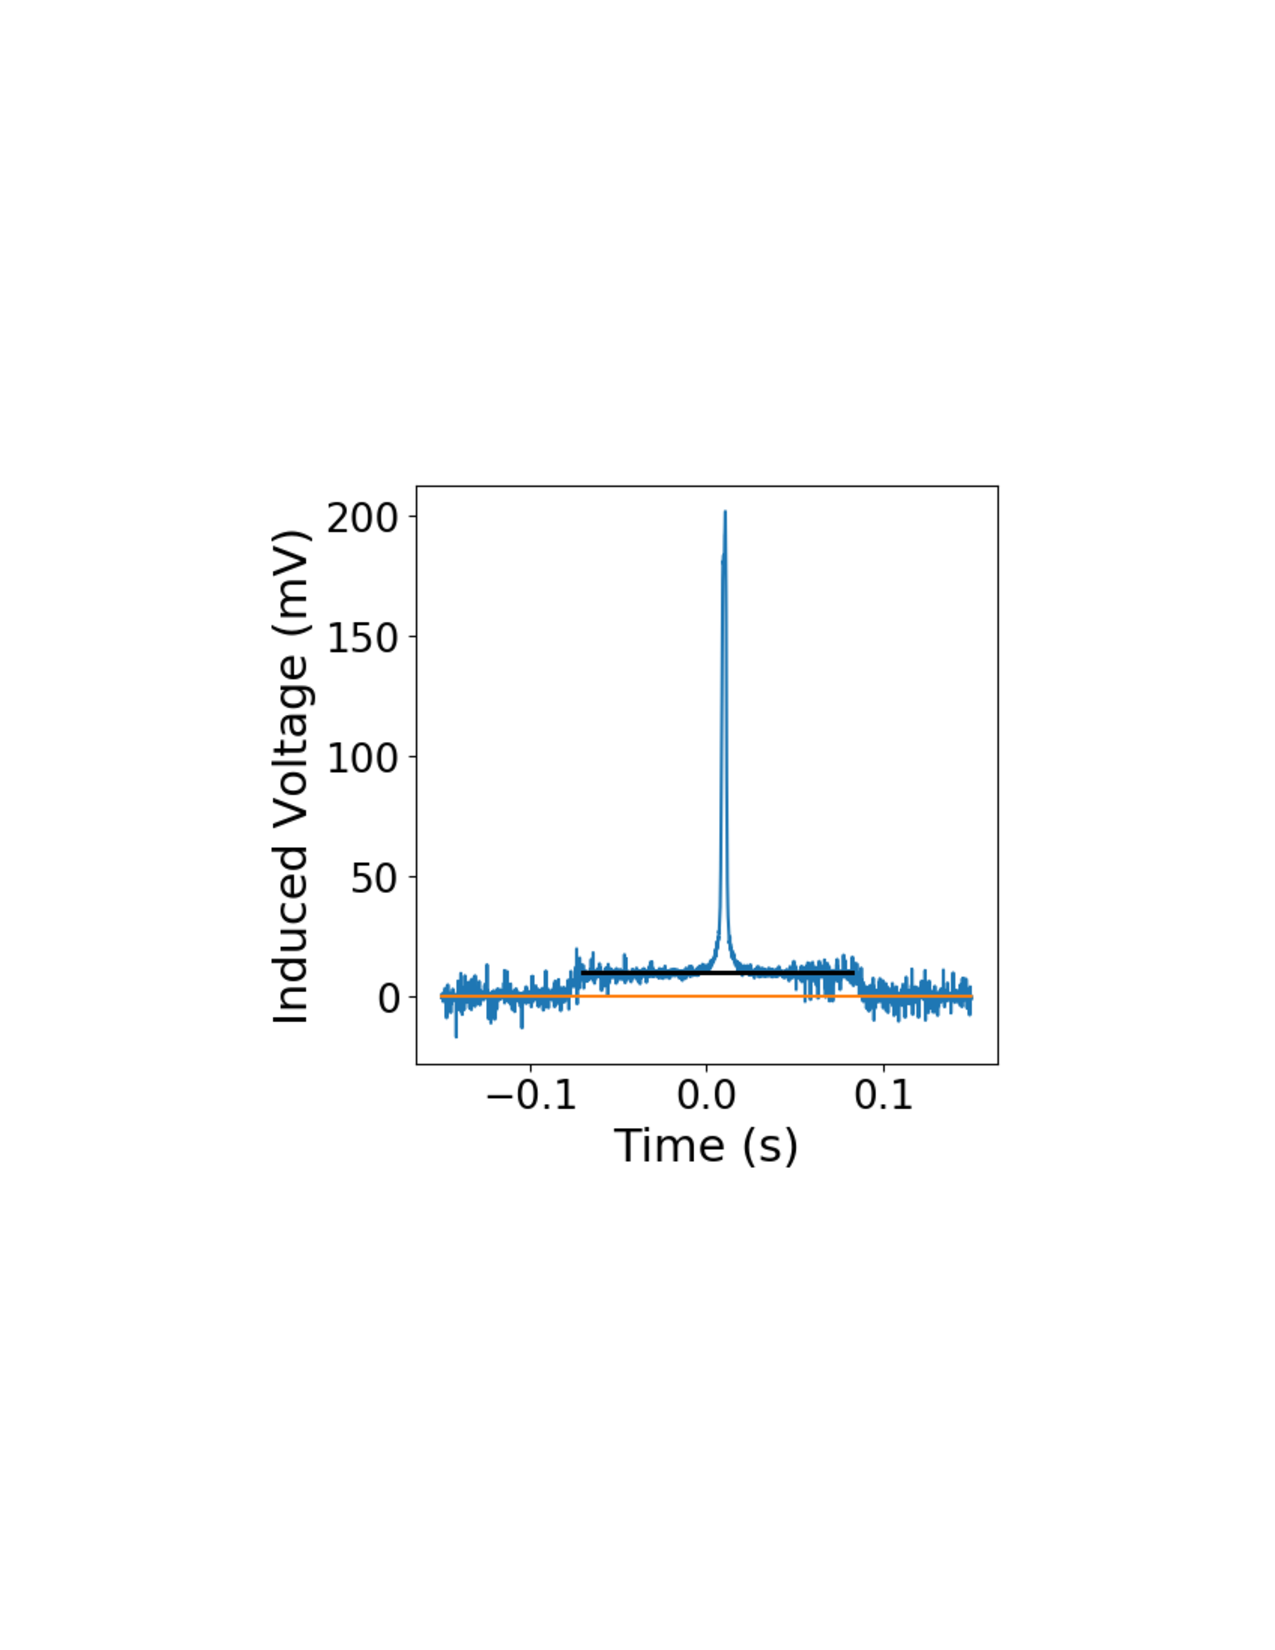
\includegraphics[width=0.45\textwidth]{11Vtgtdata.pdf}
 \end{center}
 \caption{Target pickup coil signal showing induced voltage as a function of time.  The flat part of the signal (fit with black line) corresponds 
 	to the changing applied Helmholtz field, $H$, while the sharp peak near the middle corresponds to the flip in the target magnetization.}
 \label{fig-TPolMeas}
\end{figure}

\begin{figure}[ht]
 \begin{center}
  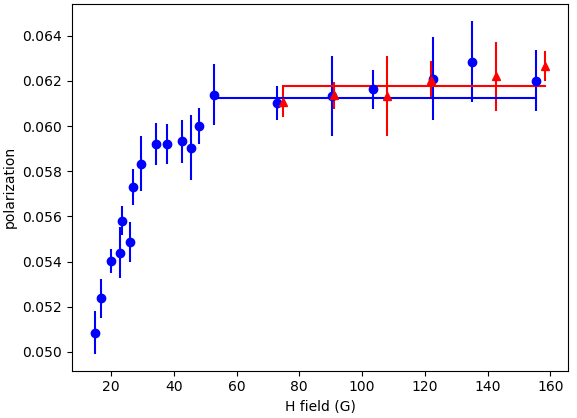
\includegraphics[width=0.45\textwidth]{PvsH0.png}
 \end{center}
	\caption{Target polarization vs.~applied magnetic field, $H$, measured with two different pickup coils. A constant fit to the flat part 
	of the curves yields values of $6.18\pm 0.03$\% for coil 1 (red diamonds) and $6.15\pm 0.04$\% for coil 2 (blue dots), where 
	uncertainties are statistical only.} 
 \label{fig-PSat}
\end{figure}

\subsection{Analyzing Power Corrections and Uncertainties}
\label{sec-PolCor}

Simulations have been performed to estimate effects due to atomic motion of the electrons and to estimate uncertainties associated with 
the polarimeter geometry. The simulation begins by randomly selecting scattering angles $\theta_{CM}$ and $\phi_{CM}$ and then transports
the scattered electrons through the magnets and towards the detectors. For events in which both electrons hit the detectors we determine an 
average analyzing power, $\langle A_{zz}\rangle$. The motion of the atomic electrons has been included in the simulation according to
Ref.~\cite{levchuk94}. Figure~\ref{fig-Azz} shows $\langle A_{zz}\rangle$ as a function of beam energy both with (orange) and without 
(blue) atomic-electron motion included in the simulation. The green curve is a fit to the points 
$\langle A_{zz}\rangle= -0.777123+(2.9249\times 10^{-3})/E$. 
The estimated relative uncertainty is $<0.01$\% and was determined by looking at variations in $\langle A_{zz}\rangle$ for reasonable 
variations in the geometry (locations of quadrupoles and detectors) and magnetic fields.
\begin{figure}[ht]
 \begin{center}
  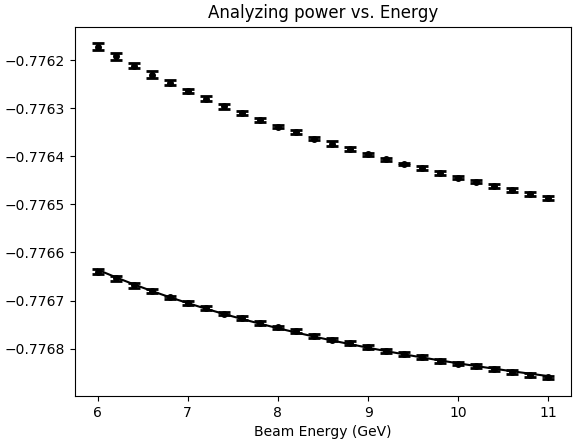
\includegraphics[width=0.45\textwidth]{Azz.png}
 \end{center}
	\caption{Average analyzing power $\langle A_{zz}\rangle$ as a function of beam energy from simulation. The upper/lower points 
	include/exclude motion of the atomic electrons. The error bars are statistical only. The curve on the lower points is a fit 
	given in the text.}
 \label{fig-Azz}
\end{figure}


%but has negligible effect due to a relatively large angular acceptance ($\delta\theta^{lab}/\theta^{lab}\approx0.14$). 


%\subsection{Spin Dance}
\subsection{Beam polarization measurements}
\label{sec-SpinDance}

Beam polarization measurements are usually done on a weekly basis or after changes to the accelerator configuration.  The shift personnel
use what is in essence a push-button GUI interface. The user selects which target to use (left or right) and the
Helmholtz coil polarity. The settings for the quadrupoles are automatically calculated based upon the beam energy. Individual M{\o}ller runs
are usually done for both targets with a statistical precision of $\pm 1.5$\%, which is slightly smaller than the total systematic uncertainty. 
The underlying software calculates the beam polarization using the beam-helicity-gated true and accidental coincidence rates from 
the M{\o}ller detectors along with the beam-helicity related charge asymmetry measured using the SLM. 
At the end of a M{\o}ller run the beam polarization is stored in the GUI and goes automatically to the electronic logbook. The scaler 
readouts during the run are stored in the run file while polarization the measurement is stored the database. 

%\begin{figure}[ht]
%\begin{center}
%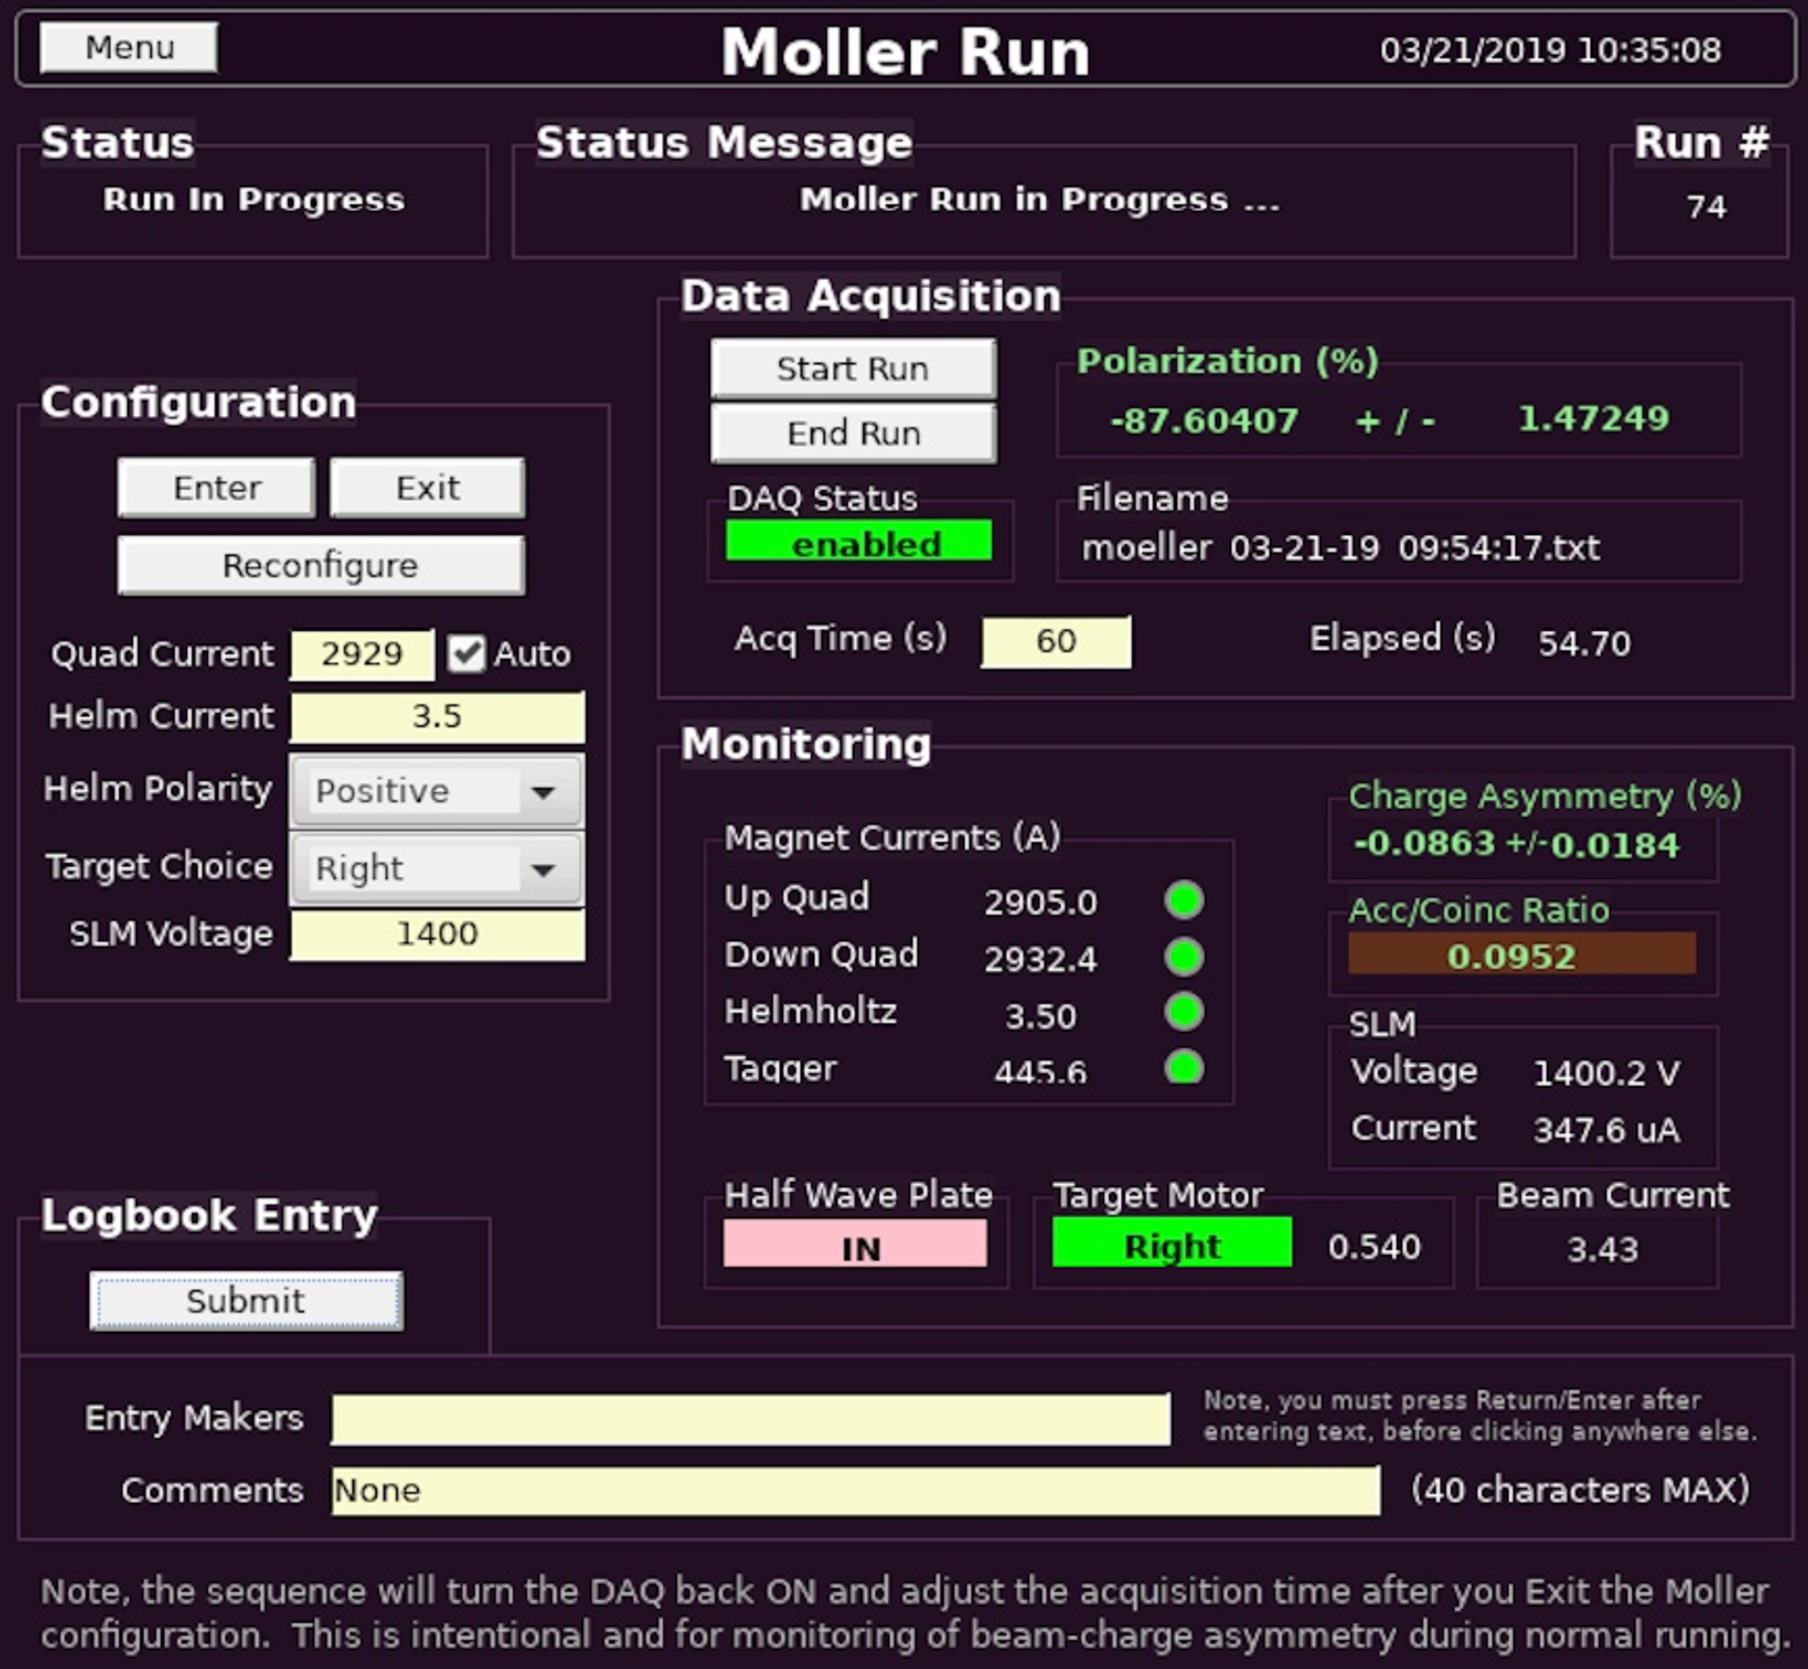
\includegraphics[width=0.475\textwidth]{moller_gui.pdf}
%	\caption{Graphical user interface for M{\o}ller polarimeter operation.}
%\label{fig:mollergui}
%\end{center}
%\end{figure}

Results of beam polarization measurements taken during the fall 2018 run period are shown in Fig.~\ref{fig:molrga}.
There are two distinct regions of beam polarization with average polarizations of $85.95\% ~\pm ~1.29\%$ and $89.22\%~\pm~2.51\%$. 
These two regions differ by settings of the angle, $\theta_W$ of the Wien filter in the injector. The initial Wien-filter angle was 
set to maximize the beam polarization in Hall B and was based on a calculation of the electron spin precession in the accelerator. 
However, the polarization in the early part of the running period fell below the expected maximum of about 90\%, which was measured 
at the injector by a Mott polarimeter, indicating an incorrectly calculated $\theta_W$ . In order to find the optimum value of $\theta_W$, 
two more M{\o}ller measurements of the beam polarization in Hall-B were performed at $\theta_W=25^\circ$ and $70^\circ$.  
The result of these measurements along with the average at $\theta_W=50^\circ$ are shown in Fig.~\ref{fig:sdance}. Fitting these three 
points with a function of $a\cos\left(\theta_W-b\right)$ (dashed curve), where $a$ and $b$ are fit parameters,  shows that the maximum
polarization of about 90\% in Hall B occurs for $\theta_W\approx 40^\circ$.
 
\begin{figure}[ht]
\begin{center}
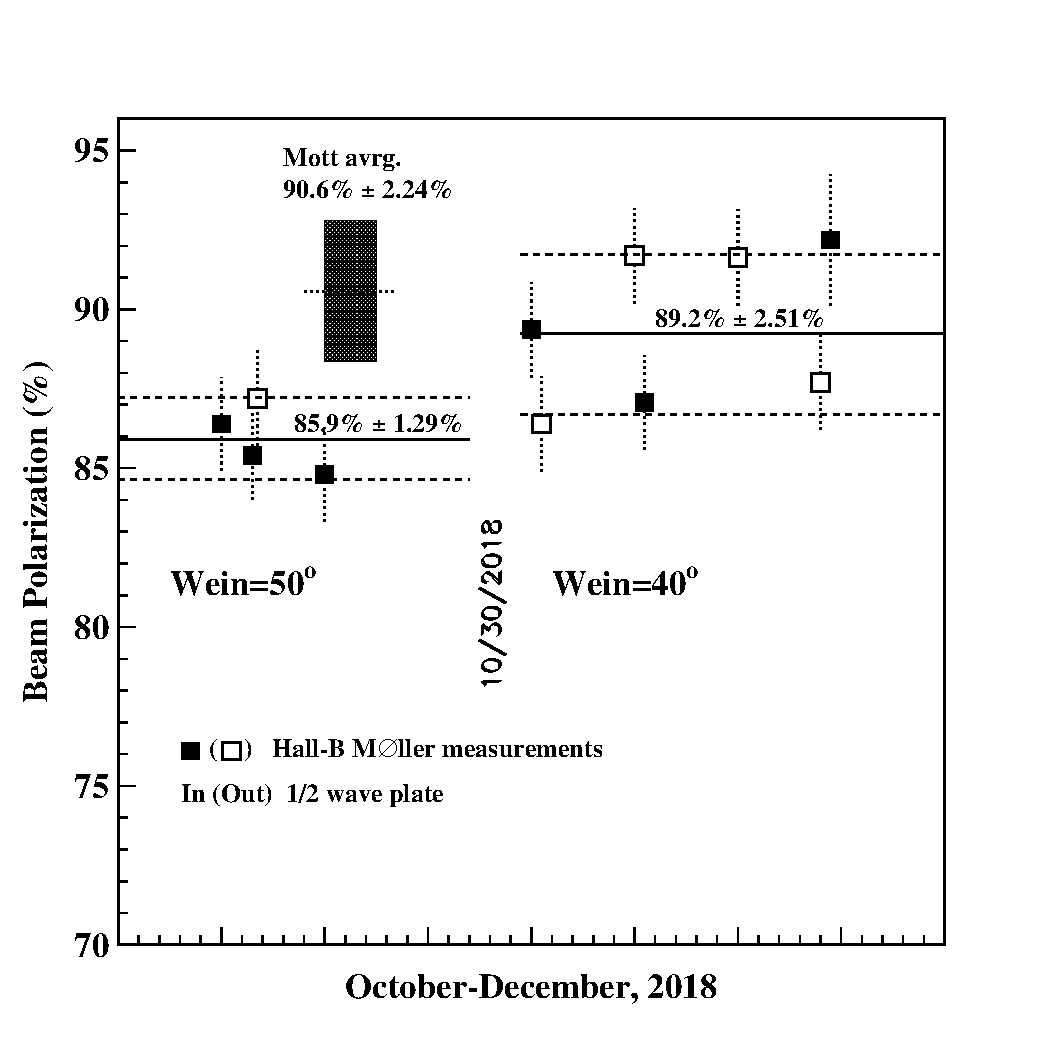
\includegraphics[width=0.5\textwidth]{Moller-RGA-2018.pdf}
	\caption{Beam polarization measured in Hall B during the fall 2018 running period. Prior to October 30 the measurements from the 
	Hall-B polarimeter (squares) averaged to $85.9\%\pm1.2\%$ (stat.), which is lower than the expected 90\% from the injector Mott 
	measurements (black band). After optimizing the Wien-filter angle the average polarization measured in Hall B was measured 
	to be $89.2\%\pm2.5\%$ (stat.). Filled and open symbols correspond to measurements made with and without a half-wave plate, 
	respectively. Error bars are statistical only.}
\label{fig:molrga}
\end{center}
\end{figure}

\begin{figure}[ht]
\begin{center}
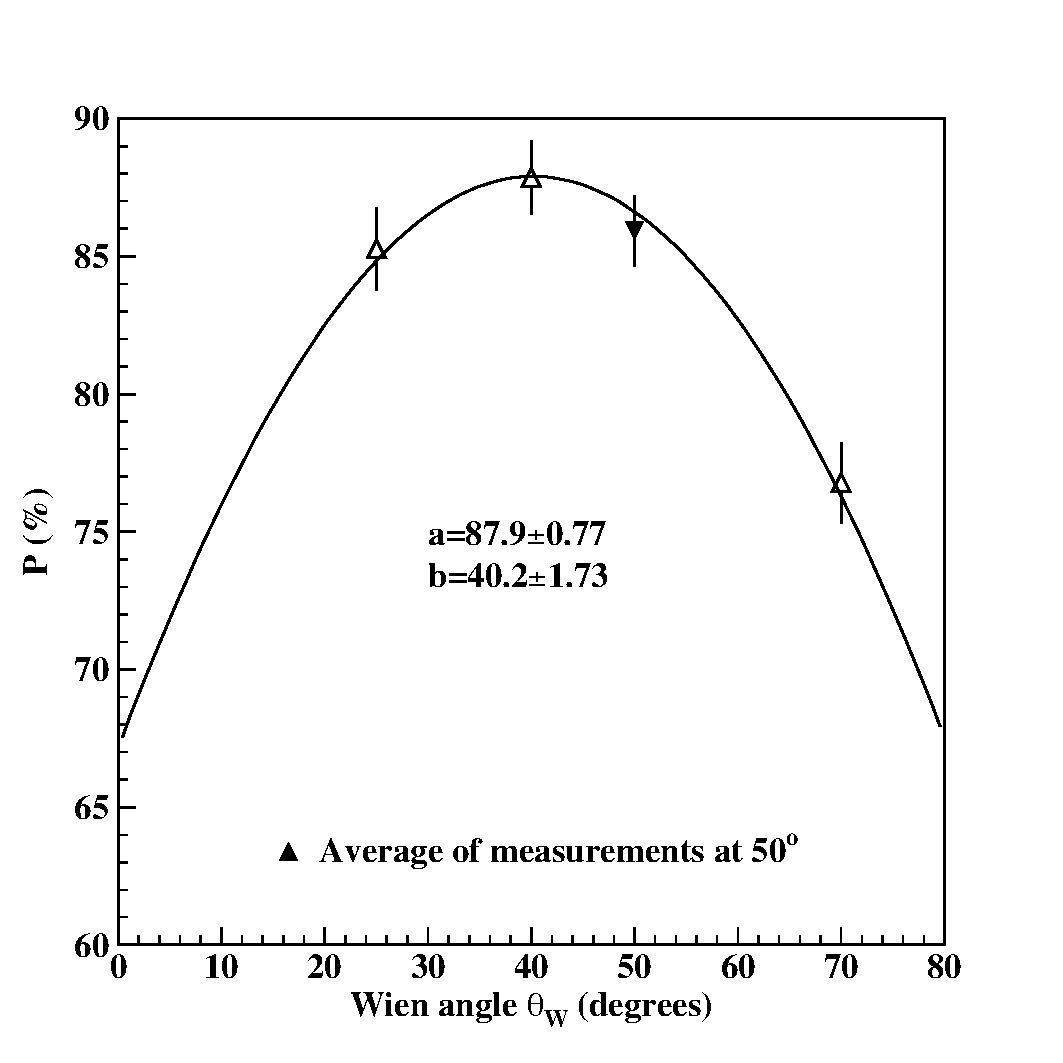
\includegraphics[width=0.5\textwidth]{Hall-B_fall_spin_dance.pdf}
	\caption{Beam polarization measurements at different Wien angle settings taken during the fall 2018 run period.  The dashed 
	curve is the cosine-function fit to the data points. The filled point is the average over all measurements with the angle set to $50^\circ$ 
	and the open points are from single measurements. Error bars are statistical only. }
\label{fig:sdance}
\end{center}
\end{figure}

Figure~\ref{fig:molrga} has two sets of Hall-B polarimeter measurements done with and without a half-wave plate. The half-wave
plate rotates the electron spin by $180^\circ$. The measurements with and without the the half-wave plate agree within statistical
uncertainties. 

